\chapter{Superspace und die Konstruktion supersymmetrischer Dynamik}

\lectureoverview{Wir bauen die Supersymmetrie aus dem kleinsten System auf, in dem sie wirken kann: einem bosonischen und einem fermionischen Oszillator gleicher Energie. Der Gegensatz zwischen ihren Gleichungen zweiter beziehungsweise erster Ordnung führt zu den Superladungen und ihrer Algebra. Anschließend deuten wir diese Algebra als Geometrie auf einem Raum mit der gewöhnlichen Koordinate (t) und den Grassmann-Koordinaten \(\theta,\bar\theta\). Superfelder fassen Bosonen, Fermionen und ein Hilfsfeld zu einem einzigen Objekt zusammen; die Berezin-Integration extrahiert eine invariante gewöhnliche Lagrange-Funktion; kovariante Ableitungen ermöglichen symmetrieverträgliche Nebenbedingungen; und die chirale Nebenbedingung liefert das erste wichtige Beispiel. In der Vorlesung werden die Vorzeichen- und Ordnungsprobleme dieses Formalismus bewusst offengelegt. Zum Schluss wird erläutert, warum die Symmetrie selbst grundlegender ist als ein Katalog von Feynman-Regeln.}

\section{Zurück zum System mit einem Modus}

Beginnen wir noch einmal mit ruhenden Fermionen und Bosonen. Wir unterdrücken alle Ortskoordinaten und Impulsbezeichnungen. In einem gegebenen Modus ist ein Quant entweder vorhanden oder nicht vorhanden; Erzeugungs- und Vernichtungsoperatoren genügen zu seiner Beschreibung. Wir schreiben \(a^\dagger,a\) für einen bosonischen Modus und \(c^\dagger,c\) für einen fermionischen Modus. Es gilt
\begin{align}
[a,a^\dagger]&=1,
&
\{c,c^\dagger\}&=1,
&
c^2=(c^\dagger)^2&=0.
\end{align}
Haben beide Quanten dieselbe Energie \(m\), so gilt bis auf eine irrelevante Vakuumkonstante
\begin{equation}
H=m\left(a^\dagger a+c^\dagger c\right).
\label{eq:l7-one-mode-hamiltonian}
\end{equation}
Der Zahloperator \(a^\dagger a\) kann jeden nichtnegativen ganzzahligen Wert annehmen, während \(c^\dagger c\) nur null oder eins sein kann. Das ist die gesamte Kinematik des Spielzeugmodells.

Diese Vereinfachung ist strategisch gewählt. Wir wollen die Operation verstehen, die ein Boson entfernt und ein Fermion einsetzt oder umgekehrt, ohne die Energie zu ändern. Bevor wir diese Operation konstruieren, übersetzen wir dasselbe System jedoch zunächst aus der Operatorsprache in die Lagrange-Formulierung.

\section{Der bosonische Oszillator}

Für das Boson führen wir eine reelle Koordinate \(\phi(t)\) ein. Ohne räumliche Abhängigkeit wird aus einem freien Skalarfeld ein gewöhnlicher harmonischer Oszillator. Der erste an die Tafel geschriebene Ausdruck lautete
\[
\frac{1}{2}\dot\phi^{,2}+\frac{1}{2}m^2\phi^2.
\]
Dieser Ausdruck ist die Summe aus kinetischer und potenzieller Energie, nicht die Lagrange-Funktion. In der Vorlesung wird das Vorzeichen sofort berichtigt:
\begin{equation}
L_B=\frac{1}{2}\dot\phi^{,2}-\frac{1}{2}m^2\phi^2.
\label{eq:l7-boson-lagrangian}
\end{equation}

\begin{figure}[H]
\centering
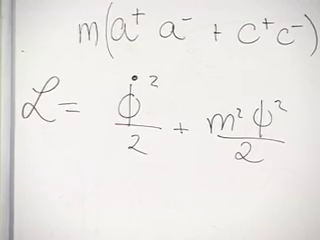
\includegraphics[width=0.62\textwidth]{lecture_07_figure_02.png}
\lectureframe{00:03:25.431}
\caption{Der Einmoden-Hamiltonoperator oberhalb der bosonischen Lagrange-Funktion. Das Bild zeigt das anfängliche Pluszeichen, bevor es mündlich zu \(T-V\) korrigiert wird.}
\end{figure}

\begin{classroomqa}
\audiencequestion{Was ist am Vorzeichen in der dargestellten Oszillator-Lagrange-Funktion falsch? \lecturetimestamp{00:04:00}}
\lecturerresponse{Die Energie ist \(T+V\), die Lagrange-Funktion jedoch \(T-V\). Der Potenzialterm muss daher ein Minuszeichen tragen. Durch die Korrektur ergibt sich statt eines exponentiellen Verhaltens die beabsichtigte harmonische Schwingung.}
\end{classroomqa}

Tatsächlich ergibt die Euler--Lagrange-Gleichung
\begin{align}
\frac{d}{dt}\frac{\partial L_B}{\partial\dot\phi}
&=\frac{\partial L_B}{\partial\phi},\\
\ddot\phi&=-m^2\phi,
\end{align}oder
\begin{equation}
\ddot\phi+m^2\phi=0.
\label{eq:l7-boson-eom}
\end{equation}
Ihre Frequenz ist \(m\), nicht \(m^2\). Die Quantisierung dieses Oszillators liefert dieselbe Zustandsleiter, die durch \(a^\dagger\) und \(a\) in Gl.~\eqref{eq:l7-one-mode-hamiltonian} beschrieben wird.

\section{Warum die fermionische Wirkung erster Ordnung ist}

Die fermionische Lagrange-Funktion sieht einfacher aus, weil sie nur eine Zeitableitung enthält. Der Grund dafür wird bereits an einem bewusst naiven Ansatz deutlich. Für eine gewöhnliche kommutierende Variable gilt
\begin{equation}
L_{\mathrm{trial}}=\phi\dot\phi
=\frac{1}{2}\frac{d}{dt}\phi^2.
\end{equation}
Dies ist eine totale Zeitableitung. Ihre Euler--Lagrange-Gleichung besagt lediglich \(\dot\phi=\dot\phi\), sodass jeder differenzierbare Pfad zulässig ist. Wird eine totale Ableitung aus der Wirkung entfernt, ändern sich die Randdaten, nicht aber die Bewegungsgleichung im Inneren.

Nun benennen wir die Variable in \(\psi\) um und erklären sie für Grassmann-ungerade. Sowohl \(\psi\) als auch \(\dot\psi\) antikommutieren. Bei einer festgelegten Wahl der Linksvariation entsteht durch das Vertauschen der ungeraden Faktoren ein Minuszeichen; derselbe formale Ansatz ergibt daher
\begin{equation}
\frac{d}{dt}\frac{\partial L_{\mathrm{trial}}}{\partial\dot\psi}
=\dot\psi,
\qquad
\frac{\partial L_{\mathrm{trial}}}{\partial\psi}
=-\dot\psi.
\end{equation}
Die Gleichung lautet somit
\begin{equation}
\dot\psi=-\dot\psi
\quad\Longrightarrow\quad
\dot\psi=0.
\label{eq:l7-constant-fermion}
\end{equation}
Der Ausdruck, der für eine kommutierende Koordinate eine Tautologie war, erhält für eine antikommutierende dynamischen Gehalt. Für einen Oszillator ist das zu viel: Er lässt nur eine konstante Lösung zu. Genau darin liegt jedoch der Hinweis, den wir brauchen.

\begin{classroomqa}
\audiencequestion{Ist die Lösung also einfach, dass \(\psi\) konstant ist? \lecturetimestamp{00:13:57}}
\lecturerresponse{Ja. Gleichung~\eqref{eq:l7-constant-fermion} ist eine echte Differentialgleichung erster Ordnung; ihre Lösung ist eine beliebige Grassmann-wertige Konstante. Ein Massenterm macht aus dieser statischen Lösung eine oszillierende.}
\end{classroomqa}

Der naheliegende Versuch, \(m\psi^2\), scheitert, weil \(\psi^2=0\). Wir brauchen zwei reelle ungerade Variablen \(\psi_1,\psi_2\) oder, gleichwertig, eine komplexe Variable und ihre konjugierte. In der Vorlesung wird die Form mit zwei reellen Variablen an der Tafel entwickelt, wobei Vorzeichen und Zweierfaktoren wiederholt überprüft werden. Eine üblich normierte komplexe Form lautet
\begin{equation}
L_F=\frac{i}{2}
\left(\bar\psi\dot\psi-\dot{\bar\psi}\psi\right)
-m\bar\psi\psi.
\label{eq:l7-fermion-lagrangian}
\end{equation}
Bis auf eine totale Ableitung ist dies \(i\bar\psi\dot\psi-m\bar\psi\psi\). Die Variation nach \(\bar\psi\) ergibt
\begin{equation}
i\dot\psi=m\psi,
\qquad
\psi(t)=\psi(0)e^{-imt}.
\label{eq:l7-fermion-eom}
\end{equation}
Für die konjugierte Gleichung gilt die entgegengesetzte Phase. Der fermionische Modus schwingt daher mit der Energie \(m\), genau wie der bosonische, obwohl seine Gleichung erster statt zweiter Ordnung ist.

\editorialnote{~\eqref{eq:l7-fermion-lagrangian} legt eine übliche Anordnung und Normierung für die probeweise Rechnung mit zwei reellen Variablen fest. In der Vorlesung wird der Faktor \(i\) eingefügt, ein Faktor zwei angepasst und das Vorzeichen einer reellen Komponente offengelassen. Diese Änderungen berühren die zentrale Schlussfolgerung nicht: Die Fermion-Kinetik ist erster Ordnung, die Masse tritt linear auf, und ein komplexes Fermion liefert eine nichtverschwindende Bilinearform.}

Dies ist der null-dimensionale Grenzfall eines vertrauten relativistischen Gegensatzes. Die Klein--Gordon-Gleichung ist zweiter Ordnung in der Zeit, die Dirac-Gleichung erster Ordnung. Wenn der Raum unterdrückt wird, entspricht das Boson einem harmonischen Oszillator und das Fermion einem komplexen Grassmann-Oszillator.

\begin{classroomqa}
\audiencequestion{Spielt die Reihenfolge eine Rolle, in der \(\psi\), \(\dot\psi\) und ihre konjugierten Größen geschrieben werden? \lecturetimestamp{00:18:58}}
\lecturerresponse{Die Zwischenausdrücke hängen von der Reihenfolge ab, weil ungerade Faktoren antikommutieren. Die physikalische Theorie hängt nicht von einer beliebigen Schreibkonvention ab, sofern durchgängig dieselbe Konvention für Links- oder Rechtsvariation, Konjugation und Integration verwendet wird. Beim Vertauschen eines ungeraden Paars ändert sich ein Vorzeichen; dieses muss dann überall sonst entsprechend angepasst werden.}
\end{classroomqa}

Aus den Gln.~\eqref{eq:l7-boson-lagrangian} und \eqref{eq:l7-fermion-lagrangian} erhalten wir eine Lagrange-Beschreibung desselben angepassten Paars, das durch Gl.~\eqref{eq:l7-one-mode-hamiltonian} dargestellt wird. Nun können wir die Symmetrie zwischen den beiden bestimmen.

\section{Superladungen und ihre Algebra}

Ein Operator, der ein Fermion entfernt und ein Boson einsetzt, lautet
\begin{equation}
Q^\dagger=\sqrt{2m}\,a^\dagger c,
\end{equation}
Sein konjugierter Operator entfernt ein Boson und setzt ein Fermion ein:
\begin{equation}
Q=\sqrt{2m}\,a c^\dagger.
\end{equation}
Die Normierung ist so gewählt, dass die Algebra ihre Standardform annimmt. Mit \(cc^\dagger=1-c^\dagger c\), \(aa^\dagger=a^\dagger a+1\) und der Tatsache, dass bosonische und fermionische Operatoren miteinander kommutieren, folgt
\begin{align}
\{Q,Q^\dagger\}
&=2m\left(ac^\dagger a^\dagger c+a^\dagger c a c^\dagger\right)\notag\\
&=2m\left[(a^\dagger a+1)c^\dagger c
+a^\dagger a(1-c^\dagger c)\right]\notag\\
&=2m\left(a^\dagger a+c^\dagger c\right)=2H.
\label{eq:l7-superalgebra}
\end{align}
Die bosonischen Operatoren lassen sich durch die fermionischen hindurchschieben. Aus derselben Nilpotenz, die die Fermionbesetzung begrenzt, folgt
\begin{equation}
Q^2=(Q^\dagger)^2=0.
\end{equation}
Schließlich gilt
\begin{equation}
[H,Q]=[H,Q^\dagger]=0.
\label{eq:l7-conserved-supercharges}
\end{equation}
Jede Superladung ändert die Bosonenzahl und die Fermionenzahl in entgegengesetzter Richtung. Bei gleichen Frequenzen heben sich daher die beiden Energieänderungen auf.

\begin{classroomqa}
\audiencequestion{Was ist \([H,Q]\)? Ist das Ergebnis proportional zu \(Q\)? \lecturetimestamp{00:25:10}}
\lecturerresponse{Nein. Das Ergebnis ist null. Ein einzelner Erzeugungs- oder Vernichtungsoperator würde bei der Kommutatorbildung mit \(H\) seine Energie beitragen, doch die bosonischen und fermionischen Beiträge in \(Q\) heben sich auf. Genau diese Aufhebung entspricht der Bedingung gleicher Energien.}
\end{classroomqa}

\begin{classroomqa}
\audiencequestion{Stand dieser Kommutator nicht schon an der Tafel? \lecturetimestamp{00:25:45}}
\lecturerresponse{Doch. Die Wiederentdeckung ist nützlich, weil sie uns zwingt, die Relation zu deuten, statt sie bloß abzuschreiben: Mit dem Hamiltonoperator zu kommutieren bedeutet, dass die Transformation eine Symmetrie ist und ihr Generator erhalten bleibt.}
\end{classroomqa}

Die Bezeichnung \emph{Ladung} verweist auf dieses Erhaltungsgesetz. Wir sollten \(Q\) jedoch nicht als gewöhnliche, gleichzeitig messbare Zahl auffassen, die einem Zustand zugeordnet ist. Sie ist Grassmann-ungerade, nilpotent und bildet einen bosonischen Zustand auf einen fermionischen ab. Die sinnvolle Aussage lautet, dass es sich um einen erhaltenen Generator handelt, der innerhalb entarteter Supermultipletts wirkt.
\editorialnote{Diese Formulierung präzisiert die Analogie aus der Vorlesung, Zustände durch ihre Energie oder elektrische Ladung zu kennzeichnen. Individuelle nichthermitesche, ungerade Superladungen sind keine gewöhnlichen Observablen mit numerischen Quantenzahlen. Ihre erhaltene Wirkung und die Darstellung der vollständigen Superalgebra liefern die passende Klassifikation.}

\section{Generatoren als Ableitungen}

Die Algebra ist kompakt, sagt für sich genommen aber noch nicht, wie sich wechselwirkende Theorien konstruieren lassen. Der nächste Schritt ist geometrischer Natur. Vertraute Symmetrieerzeuger wirken bereits als Differentialoperatoren. In der Konvention der Vorlesung gilt
\begin{equation}
H=i\frac{\partial}{\partial t},
\qquad
P=-i\frac{\partial}{\partial x}.
\end{equation}

\begin{figure}[H]
\centering
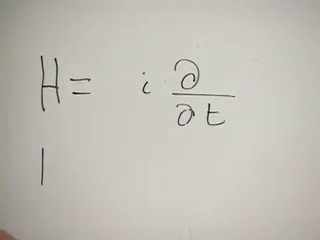
\includegraphics[width=0.50\textwidth]{lecture_07_figure_03.png}
\lectureframe{00:28:12.720}
\caption{Der Hamiltonoperator, dargestellt als Generator der Zeittranslationen.}
\end{figure}

Der Drehimpuls ist ebenfalls das Produkt aus einer Koordinate und einer Ableitung. Wenn Superladungen ungerade Generatoren sind, liegt die Frage nahe, ob sie sich durch Ableitungen nach ungeraden Koordinaten darstellen lassen. Dazu erweitern wir die Zeitachse zum Superspace
\begin{equation}
(t,\theta,\bar\theta),
\qquad
\theta^2=\bar\theta^2=0,
\qquad
\theta\bar\theta=-\bar\theta\theta.
\end{equation}
Felder auf diesem Raum hängen von einer gewöhnlichen Zeit und einem Paar konjugierter Grassmann-Koordinaten ab.

In der Vorlesung wird bewusst gezeigt, wie tückisch die Vorzeichen sind. Ein Vorzeichen aus der komplexen Konjugation, eines vom Verschieben eines ungeraden Parameters und eines aus der Wahl von Links- statt Rechtsableitungen stehen für verschiedene Operationen. Statt einander widersprechende Zwischenstände an der Tafel zu übernehmen, legen wir nun eine Konvention fest: Alle ungeraden Ableitungen sind Linksableitungen, und es gilt
\begin{equation}
q=\partial_\theta+i\bar\theta\partial_t,
\qquad
\bar q=\partial_{\bar\theta}+i\theta\partial_t.
\label{eq:l7-differential-supercharges}
\end{equation}
Dann folgt
\begin{equation}
q^2=\bar q^{,2}=0,
\qquad
\{q,\bar q\}=2i\partial_t=2H.
\label{eq:l7-differential-algebra}
\end{equation}
Der Faktor zwei entsteht durch zwei gemischte Terme: \(\{\partial_\theta,\theta\}=1\) und \(\{\partial_{\bar\theta},\bar\theta\}=1\). Enthielten die Generatoren nur \(\partial_\theta\) und \(\partial_{\bar\theta}\), wäre ihr Antikommutator null und könnte den Hamiltonoperator nicht reproduzieren.

\begin{classroomqa}
\audiencequestion{Müssen die beiden Zeitableitungsterme in \(q\) und \(\bar q\) dasselbe Vorzeichen haben? \lecturetimestamp{00:31:01}}
\lecturerresponse{Sie müssen so gewählt werden, dass der gemischte Antikommutator \(2H\) ergibt. Möglich ist sowohl eine Konvention mit durchgehendem Pluszeichen als auch die konsistent konjugierte Alternative. Die Rechnung, nicht der optische Eindruck des Symbols \(i\), legt die relativen Vorzeichen fest.}
\end{classroomqa}

Im Hörsaal werden die Vorzeichen wiederholt überprüft, bis daraus ein Scherz wird: Auf dem Weg zur Arbeit scheinen sie sich zu ändern. Der Scherz trifft den Punkt. Wenn ein Grassmann-Parameter an einer Koordinate vorbeigeschoben wird, kann sich ein Vorzeichen ändern, auch wenn sich an der physikalischen Konvention nichts geändert hat. Gleichung~\eqref{eq:l7-differential-supercharges} ist die feste Referenz für alles Weitere.

\subsection{Supersymmetrie als Koordinatenverschiebung}

Seien \(\xi,\bar\xi\) infinitesimale ungerade Parameter. Die Wirkung auf ein Superfeld mit
\begin{equation}
\delta_\xi=\xi q+\bar\xi\bar q
\end{equation}
ist in der obigen Konvention gleich der infinitesimalen Koordinatentransformation
\begin{align}
\theta&\longrightarrow\theta+\xi,\\
\bar\theta&\longrightarrow\bar\theta+\bar\xi,\\
t&\longrightarrow t+i\left(\xi\bar\theta+\bar\xi\theta\right).
\label{eq:l7-coordinate-shift}
\end{align}
Die Änderung eines skalaren Superfelds lautet daher
\begin{equation}
\delta_\xi\Phi
=\left(\xi\partial_\theta+\bar\xi\partial_{\bar\theta}
+i\xi\bar\theta\partial_t+i\bar\xi\theta\partial_t\right)\Phi
=\left(\xi q+\bar\xi\bar q\right)\Phi.
\end{equation}
Das ist der geometrische Gehalt der Supersymmetrie: eine Translation in ungeraden Richtungen, die an eine Translation in der gewöhnlichen Zeit gekoppelt ist. Zwei ungerade Verschiebungen schließen sich gemäß Gl.~\eqref{eq:l7-differential-algebra} zu einer Zeittranslation zusammen.

\begin{classroomqa}
\audiencequestion{Könnte das umstrittene Minuszeichen eine Bewegung rückwärts in der Zeit darstellen? \lecturetimestamp{00:58:13}}
\lecturerresponse{Eine andere Vorzeichenkonvention kann die dargestellte infinitesimale Zeitverschiebung umkehren; damit wird jedoch kein eigener physikalischer Prozess rückwärts in der Zeit eingeführt. Entscheidend ist, dass Koordinatentransformation und Differentialgeneratoren dieselbe Algebra erfüllen.}
\end{classroomqa}

\begin{classroomqa}
\audiencequestion{Lässt sich diese erweiterte Zeit physikalisch realisieren, oder dient sie nur der formalen Buchführung? \lecturetimestamp{00:58:23}}
\lecturerresponse{In einem nützlichen Sinn dient sie der Buchführung: Sie fasst die Algebra geometrisch zusammen. Diese Darstellung wird jedoch physikalisch wertvoll, sobald Wechselwirkungen eingeführt werden. Der Superspace liefert einen systematischen Kalkül, mit dem sich Lagrange-Funktionen konstruieren lassen, die in jedem Schritt die Boson--Fermion-Symmetrie bewahren, ähnlich wie die Tensorrechnung uns dabei hilft, Lorentz-Skalare zu bilden.}
\end{classroomqa}

\section{Superfelder und die Hilfskomponente}

Da es nur zwei ungerade Koordinaten gibt, bricht die Entwicklung eines geraden Superfelds nach endlich vielen Termen ab:
\begin{equation}
\Phi(t,\theta,\bar\theta)
=\phi(t)+\bar\theta\psi(t)+\bar\psi(t)\theta
+D(t)\bar\theta\theta.
\label{eq:l7-superfield}
\end{equation}
Die Koeffizienten der geraden Monome, \(\phi\) und \(D\), sind bosonisch; die Koeffizienten der ungeraden Monome, \(\psi\) und \(\bar\psi\), sind fermionisch. Kein Term mit \(\theta^2\), \(\bar\theta^2\) oder höherer Ordnung bleibt übrig. Die Zeitabhängigkeit lassen wir unentwickelt, denn eine gewöhnliche Taylor-Reihe in \(t\) bräche nicht ab und wäre hier zwecklos.

\begin{classroomqa}
\audiencequestion{Was ist die Komponente \(D(t)\) im obersten Term? \lecturetimestamp{00:41:46}}
\lecturerresponse{An dieser Stelle ist sie einfach der letzte bosonische Koeffizient in der endlichen Entwicklung. In der Komponentenwirkung hat sie normalerweise keinen kinetischen Term und wird durch eine algebraische Bewegungsgleichung eliminiert; daher heißt sie Hilfsfeld. In der Vorlesung wird scherzhaft ``D wie Dummy'' vorgeschlagen. Das bringt seine nichtdynamische Rolle zum Ausdruck, ist aber nicht die historische Herleitung der Bezeichnung.}
\end{classroomqa}

Das Superfeld ist ein einzelnes Objekt, während \(\phi,\psi,\bar\psi,D\) seine Komponenten sind. Eine Supersymmetrietransformation mischt sie. In diesem strukturellen Sinn sind ein Boson und ein Fermion ähnlich miteinander verknüpft wie die \(x\)- und \(y\)-Komponenten eines Vektors durch eine Rotation, auch wenn sich Grassmann-Richtungen nicht als gewöhnliche Achsen veranschaulichen lassen.

\section{Die Superwirkung und die oberste Komponente}

Um Bewegungsgleichungen zu erhalten, brauchen wir eine Wirkung. In der gewöhnlichen Feldtheorie bildet man eine skalare Lagrange-Funktion und integriert sie über die Raumzeit. Das entsprechende Gebilde lautet hier
\begin{equation}
S=\int dt\,d\theta\,d\bar\theta\;\Lambda
\bigl(\Phi,\text{ superspace derivatives of }\Phi\bigr),
\label{eq:l7-superaction}
\end{equation}
Dabei ist \(\Lambda\) ein gerades Superfeld. Die Berezin-Integration ist algebraisch. Wir legen fest:
\begin{equation}
\int d\theta\,d\bar\theta\;\bar\theta\theta=1.
\end{equation}
Wenn also
\begin{equation}
\Lambda=A+\bar\theta B+\bar B\theta+C\bar\theta\theta,
\end{equation}
gilt, dann ist
\begin{equation}
\int d\theta\,d\bar\theta\;\Lambda=C.
\label{eq:l7-top-component}
\end{equation}
Die Integration über die ungeraden Koordinaten extrahiert die oberste Komponente und lässt eine gewöhnliche Lagrange-Funktion zurück, die über die Zeit zu integrieren ist.

Warum ist das Ergebnis invariant? Eine Supersymmetrievariation verschiebt die Integrationsvariablen. Die Variation der obersten Komponente ist eine gewöhnliche totale Zeitableitung, während totale Ableitungen nach ungeraden Koordinaten bei der Berezin-Integration verschwinden. Unter geeigneten Randbedingungen bleibt die Wirkung unverändert. Dies entspricht im Superspace dem Vorgehen, vor der Integration über die Raumzeit einen Lorentz-Skalar zu bilden.

\section{Superfelder multiplizieren}

Am einfachsten erhält man aus einem Superfeld ein neues, indem man es mit sich selbst multipliziert. Ausgehend von Gl.~\eqref{eq:l7-superfield} verschwinden alle Terme, die \(\theta^2\) oder \(\bar\theta^2\) enthalten. Wir behalten die Reihenfolge \(\bar\theta\theta\) bei und schreiben die gestrichenen Komponentenfelder nach links:
\begin{align}
\Phi^2
={}&\phi^2
+2\phi\bar\theta\psi
+2\phi\bar\psi\theta\notag\\
&+\left(2\phi D-2\bar\psi\psi\right)\bar\theta\theta.
\label{eq:l7-superfield-square}
\end{align}

\begin{figure}[H]
\centering
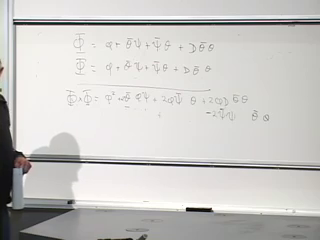
\includegraphics[width=0.82\textwidth]{lecture_07_figure_05.png}
\lectureframe{01:07:57.844}
\caption{Das komponentenweise Produkt der Superfelder und die Zusammenstellung seiner Terme mit \(\bar\theta\theta\).}
\end{figure}

Die beiden Terme \(\phi D\) und \(D\phi\) addieren sich, weil beide Felder gerade sind. Auch die beiden fermionischen Kreuzterme addieren sich nach dem jeweiligen Umordnen, doch ihr gemeinsames Vorzeichen ist negativ:
\begin{equation}
(\bar\theta\psi)(\bar\psi\theta)
+(\bar\psi\theta)(\bar\theta\psi)
=-2\bar\psi\psi\,\bar\theta\theta.
\end{equation}
Die Integration des Quadrats über die ungeraden Koordinaten ergibt
\begin{equation}
\int d\theta\,d\bar\theta\;\Phi^2
=2\phi D-2\bar\psi\psi.
\end{equation}
Dieser Term ist konstruktionsbedingt supersymmetrisch, aber noch keine kinetische Lagrange-Funktion. Er enthält keine Zeitableitungen.

Anschließend schlägt die Vorlesung \(\Phi^3\), \(\Phi^4\) und \(\Phi^n\) als Übungsaufgaben vor. Es gibt eine kompakte Regel. Für jede gewöhnliche Funktion \(W\) gilt
\begin{equation}
\left.W(\Phi)\right|_{\bar\theta\theta}
=W'(\phi)D-W''(\phi)\bar\psi\psi.
\label{eq:l7-function-top-component}
\end{equation}
Für \(W(\phi)=\phi^2\) ergibt sich daraus Gl.~\eqref{eq:l7-superfield-square}; für \(W(\phi)=\phi^n\) erhält man
\begin{equation}
\left.\Phi^n\right|_{\bar\theta\theta}
=n\phi^{n-1}D-n(n-1)\phi^{n-2}\bar\psi\psi.
\end{equation}
\editorialnote{Die Vorlesung stellt die \(n\)-te Potenz als Übungsaufgabe und nennt die erwarteten Arten von Termen. Gleichung~\eqref{eq:l7-function-top-component} enthält die vollständige Regel in der festgelegten Anordnung.}

Nun fragt der Dozent, ob der Hörsaal erschöpft sei. Das Publikum verneint; er selbst sagt, er sei es. Dieser Austausch ist mehr als eine komische Auflockerung. Potenzen von Superfeldern sind einfach, weil ihre Entwicklung abbricht. Bei Ableitungen und Nebenbedingungen wird die Vorzeichenbuchhaltung jedoch wirklich anspruchsvoll.

\section{Welche Ableitungen sind mit der Supersymmetrie verträglich?}

Bevor wir dem nächsten Argument an der Tafel folgen, ist eine Korrektur nötig. Die gewöhnliche Zeitableitung ist unproblematisch:
\begin{equation}
[\partial_t,q]=[\partial_t,\bar q]=0.
\end{equation}
Folglich transformiert \(\partial_t\Phi\) genau dann wie ein Superfeld, wenn \(\Phi\) dies tut. Heikel sind die bloßen ungeraden Ableitungen \(\partial_\theta\Phi\) und \(\partial_{\bar\theta}\Phi\), denn sie antikommutieren nicht mit beiden Superladungen. Für Nebenbedingungen und manifest supersymmetrische Komponentenkonstruktionen benötigen wir modifizierte ungerade Ableitungen.
\editorialnote{Die mündliche Behauptung, eine Zeitableitung ergebe kein weiteres Superfeld, ist in der hier verwendeten Konvention nicht richtig. Da \(\partial_t\) mit beiden Superladungen kommutiert, ist sie kovariant. Die anschließende Konstruktion modifizierter ungerader Ableitungen bleibt notwendig und ist der eigentliche mathematische Punkt der Vorlesung.}

\subsection{Die Analogie zum ``magischen Feld''}

Die Vorlesung veranschaulicht das Kriterium anhand gewöhnlicher Rotationen. Sei \(f(x,y)\) eine Funktion mit der Eigenschaft
\begin{equation}
\partial_y f=0.
\label{eq:l7-magic-constraint}
\end{equation}
Eine solche Funktion nennen wir ``magisches Feld.'' Sie hängt von \(x\), aber nicht von \(y\) ab. Bleibt die Klasse der magischen Felder unter Rotationen erhalten? Für
\begin{equation}
L_z=-i\left(x\partial_y-y\partial_x\right),
\end{equation}
finden wir
\begin{equation}
[\partial_y,L_z]=i\partial_x\neq0.
\end{equation}
Daher erhält \(L_z f\) im Allgemeinen eine \(y\)-Abhängigkeit, selbst wenn \(f\) ursprünglich Gl.~\eqref{eq:l7-magic-constraint} genügt. Die Nebenbedingung ist nicht rotationsinvariant.

Die allgemeine Schlussfolgerung ist einfach. Erfüllt ein Feld \(C\Phi=0\) und wird eine Symmetrie durch \(G\) erzeugt, so bleibt das transformierte Feld genau dann der Nebenbedingung unterworfen, wenn der graduierte Kommutator von \(C\) und \(G\) verschwindet. Für zwei ungerade Operatoren ist der graduierte Kommutator ein Antikommutator.

\begin{classroomqa}
\audiencequestion{Wann ist eine Nebenbedingung für ein Feld mit einer Symmetrie verträglich? \lecturetimestamp{01:17:56}}
\lecturerresponse{Wenn der Nebenbedingungsoperator mit den Symmetriegeneratoren graduiert kommutiert. Dann lässt sich \(C(G\Phi)\) an \(G\) vorbeischieben und zu \(G(C\Phi)=0\) vereinfachen. Das Rotationsbeispiel scheitert, weil \(\partial_y\) nicht mit dem Rotationsgenerator kommutiert.}
\end{classroomqa}

\subsection{Kovariante ungerade Ableitungen}

Mit den durch Gl.~\eqref{eq:l7-differential-supercharges} festgelegten Superladungen definieren wir
\begin{equation}
\mathcal D=\partial_\theta-i\bar\theta\partial_t,
\qquad
\bar{\mathcal D}=\partial_{\bar\theta}-i\theta\partial_t.
\label{eq:l7-covariant-derivatives}
\end{equation}
Nur das Vorzeichen des Zeitableitungsterms ändert sich. Eine direkte Rechnung ergibt
\begin{align}
\{\mathcal D,q\}
&=\{\mathcal D,\bar q\}
=\{\bar{\mathcal D},q\}
=\{\bar{\mathcal D},\bar q\}=0,\\
\{\mathcal D,\bar{\mathcal D}\}&=-2i\partial_t.
\label{eq:l7-covariant-algebra}
\end{align}
Die beiden potenziell von null verschiedenen Kreuzterme heben sich auf. Dies ist das ungerade Analogon einer kovarianten Ableitung: Sie differenziert und bewahrt dabei das Transformationsgesetz.

In der Vorlesung bezeichnet \(D\) sowohl die Hilfskomponente als auch diese Ableitung. Wir reservieren \(D(t)\) für die Komponente und verwenden das kalligrafische \(\mathcal D\) für den Operator.

\section{Die chirale Nebenbedingung}

Nun können wir eine nichttriviale Nebenbedingung auferlegen, die unter Supersymmetrie erhalten bleibt:
\begin{equation}
\bar{\mathcal D}\Phi=0.
\label{eq:l7-chiral-constraint}
\end{equation}
Ein solches Feld heißt chiral. Ist ein Feld vor einer Supersymmetrietransformation chiral, dann gilt
\begin{equation}
\bar{\mathcal D}(q\Phi)
=-q(\bar{\mathcal D}\Phi)=0,
\qquad
\bar{\mathcal D}(\bar q\Phi)
=-\bar q(\bar{\mathcal D}\Phi)=0.
\end{equation}
Das gesamte transformierte Superfeld bleibt somit in der eingeschränkten Klasse. Anders als die Bedingung für ein magisches Feld ist die Chiralität mit der Symmetrie verträglich.

Um die Nebenbedingung zu lösen, führen wir eine verschobene Zeitkoordinate ein:
\begin{equation}
\tau=t+i\bar\theta\theta.
\label{eq:l7-chiral-time}
\end{equation}
Da wir Linksableitungen verwenden, gilt
\begin{equation}
\partial_{\bar\theta}\tau=i\theta,
\end{equation}
und somit
\begin{equation}
\bar{\mathcal D}F(\tau,\theta)
=\left(\partial_{\bar\theta}-i\theta\partial_t\right)F(\tau,\theta)
=i\theta\partial_\tau F-i\theta\partial_\tau F=0.
\end{equation}
Das allgemeine lokale chirale Superfeld hängt daher von \(\bar\theta\) nur über \(\tau\) ab:
\begin{equation}
\Phi_{\mathrm{ch}}(\tau,\theta)
=\phi(\tau)+\bar\psi(\tau)\theta.
\label{eq:l7-chiral-field-tau}
\end{equation}

\begin{classroomqa}
\audiencequestion{Ist die Abhängigkeit von \(\tau\) und \(\theta\) die einzige Form, die der chiralen Nebenbedingung genügt? \lecturetimestamp{01:32:35}}
\lecturerresponse{Lokal: ja. Die Differentialgleichung \(\bar{\mathcal D}\Phi=0\) besagt genau, dass sich die unabhängige Abhängigkeit von \(\bar\theta\) in die verschobene Koordinate \(\tau=t+i\bar\theta\theta\) aufnehmen lässt. Die verbleibende endliche Entwicklung ist eine Funktion von \(\tau\) zuzüglich eines Terms proportional zu \(\theta\).}
\end{classroomqa}

Entwickeln wir wieder in der ursprünglichen Zeitkoordinate,
\begin{align}
\phi(\tau)
&=\phi(t)+i\bar\theta\theta\dot\phi(t),\\
\bar\psi(\tau)\theta
&=\bar\psi(t)\theta,
\end{align}
denn die Korrektur in der zweiten Zeile enthält \(\theta^2\). Daher gilt
\begin{equation}
\Phi_{\mathrm{ch}}(t,\theta,\bar\theta)
=\phi(t)+\bar\psi(t)\theta
+i\bar\theta\theta\dot\phi(t).
\label{eq:l7-chiral-field-components}
\end{equation}

\begin{classroomqa}
\audiencequestion{Müsste die Taylor-Entwicklung von \(\phi(t+i\bar\theta\theta)\) nicht einen Term zweiter Ordnung enthalten? \lecturetimestamp{01:33:51}}
\lecturerresponse{Nein. Die erste Korrektur ist \(i\bar\theta\theta\dot\phi\), und jede Korrektur höherer Ordnung enthält \((\bar\theta\theta)^2=0\). Das Publikum bemerkt es sofort: Die Nilpotenz hat bereits die ersten beiden Terme geliefert und die Reihe beendet.}
\end{classroomqa}

Darin liegt die Sparsamkeit der Chiralität. Das uneingeschränkte Superfeld aus Gl.~\eqref{eq:l7-superfield} hat zwei bosonische und zwei fermionische Komponentenplätze. In diesem minimalen eindimensionalen Beispiel entfernt die chirale Bedingung den unabhängigen Hilfsfeldplatz und bindet die oberste Komponente an \(\dot\phi\).

\section{Die Rechnung, die zu Recht abgebrochen wird}

Der naheliegende nächste Schritt ist, das chirale Feld mit seinem konjugierten Feld zu kombinieren und über den Superspace zu integrieren. Die Entwicklung des konjugierten Felds wird begonnen, und ein Zuhörer fragt, ob sich die Reihenfolge \(\theta\bar\theta\) bei der Konjugation umkehren muss. An diesem Punkt erscheinen die Vorzeichen nicht mehr verlässlich. Statt zu bluffen, wird die Rechnung abgebrochen.

\begin{classroomqa}
\audiencequestion{Können wir schon das Ergebnis hören, auch wenn die Multiplikation mit dem konjugierten Feld vertagt wird? \lecturetimestamp{01:37:30}}
\lecturerresponse{Ja. Werden Vorzeichen und Konjugation konsistent behandelt, liefert ein Superspace-Ausdruck aus einem chiralen Feld und seinem konjugierten Feld die gewünschten gewöhnlichen bosonischen und fermionischen kinetischen Terme. Für diese Vorlesung ist das Konstruktionsprinzip entscheidend, nicht eine unzuverlässige Schlusszeile aus einer ermüdeten Rechnung.}
\end{classroomqa}

Der Abbruchpunkt sollte sichtbar bleiben. Der Formalismus verzeiht keine Nachlässigkeit: Ein falsch platziertes ungerades Feld ändert ein Vorzeichen, und dieselbe Konvention muss bei Konjugation, Ableitung, Multiplikation und Integration konsequent beibehalten werden. Geht diese Kette verloren, muss sie repariert werden, bevor die Rechnung weitergeht. In einer Standardkonvention wird die vertraute kinetische Wirkung aus einem konjugierten Produkt gebildet; die detaillierte Komponentenreduktion gehört jedoch in die nächste saubere Rechnung und nicht in die Rekonstruktion einer unvollendeten Tafelzeile.

\section{Warum die Symmetrie die eigentliche Pointe ist}

Eine supersymmetrische Lagrange-Funktion stellt ein Boson und ein Fermion nicht bloß nebeneinander. Sie legt ihre Massen und Wechselwirkungen so fest, dass sie eine Darstellung der Superalgebra bilden. In einem exakt supersymmetrischen Vakuum haben die Mitglieder eines Supermultipletts gleiche Massen. Ihre Schleifenbeiträge sind miteinander verknüpft, und bosonische sowie fermionische ultraviolette Effekte heben sich genau in den von der Symmetrie vorgegebenen Kombinationen auf.

Darum ist der Konstruktionsformalismus wichtig. Man könnte Feynman-Vertices auflisten und die Aufhebungen diagrammweise überprüfen; dann sähen sie jedoch zufällig aus. Die Supersymmetrie erklärt sie so, wie die Lorentz-Symmetrie erklärt, dass sich Streuamplituden in jedem Inertialsystem konsistent transformieren.

\editorialnote{Exakte Supersymmetrie bedeutet nicht, dass jede einzelne Selbstenergiekorrektur verschwindet. Sie verknüpft Renormierungen und beseitigt bestimmte ultraviolette Empfindlichkeiten; Aussagen über Nicht-Renormierung hängen von der jeweiligen Größe, der Dimension und dem Ausmaß der Supersymmetrie ab. Die weit gefasste Aussage der Vorlesung über Aufhebungen wird in dieser qualifizierten Form beibehalten.}

\begin{classroomqa}
\audiencequestion{Wie schreibt man ``chiral''? \lecturetimestamp{01:39:48}}
\lecturerresponse{C-H-I-R-A-L. Das Wort bezeichnet die Nebenbedingung \(\bar{\mathcal D}\Phi=0\); es meint nicht die gewöhnliche geometrische Händigkeit eines Objekts im dreidimensionalen Raum, auch wenn die Bezeichnung auf die links- und rechtshändige Struktur relativistischer Spinoren zurückgeht.}
\end{classroomqa}

\begin{classroomqa}
\audiencequestion{Könnte man die Lagrange-Funktion umgehen und direkt zu supersymmetrischen Feynman-Regeln übergehen? \lecturetimestamp{01:40:00}}
\lecturerresponse{Man kann die Regeln durchaus angeben; dann wirken jedoch die Beziehungen zwischen den Kopplungen und die daraus folgenden Aufhebungen wie unerklärte Zufälle. Der tiefere Gehalt ist die verallgemeinerte Raumzeit-Symmetrie. Die Lagrange-Funktion oder eine gleichwertige invariante Formulierung macht diesen Grund sichtbar und liefert systematisch die Regeln.}
\end{classroomqa}

Angenommen, jede Störungsordnung ergäbe zufällig lorentzinvariante Amplituden, obwohl keine Lorentztransformationen erwähnt worden wären. Nach genügend vielen Rechnungen würden wir eine Erklärung verlangen. Sie läge in der Raumzeitsymmetrie, die alle Ordnungen zugleich ordnet. Die Rolle des Supersraums ist vergleichbar: Verschiebungen in \(\theta,\bar\theta\) mischen bosonische und fermionische Komponenten, und ihre Algebra schließt sich auf Translationen in der Raumzeit.

\begin{classroomqa}
\audiencequestion{Sollten auch die gewöhnlichen Raumkoordinaten, wie die Grassmann-Koordinaten, in einer endlichen Potenzreihe entwickelt werden? \lecturetimestamp{01:44:55}}
\lecturerresponse{Nein. Eine Potenzreihe in einer gewöhnlichen Koordinate bricht nicht ab und ist gewöhnlich keine natürliche Zerlegung. Eine Fourier-Transformation ist nützlicher, weil sie ein Feld in Wellen und Impulse zerlegt. Die Entwicklung in \(\theta\) ist gerade deshalb besonders, weil sie aufgrund der Nilpotenz endlich ist.}
\end{classroomqa}

\begin{classroomqa}
\audiencequestion{Wenn am LHC ein neues Teilchen entdeckt würde, woran könnten wir erkennen, dass es ein Superpartner und nicht bloß ein bislang unbekanntes Teilchen ist? \lecturetimestamp{01:45:42}}
\lecturerresponse{Die Supersymmetrie sagt korrelierte Quantenzahlen und Wechselwirkungen voraus, nicht nur einen zusätzlichen Zustand. Die Spins unterscheiden sich um eine halbe Einheit, die Eichladungen stehen in Beziehung zueinander, und viele kubische und quartische Kopplungen werden durch weniger unabhängige Parameter bestimmt als in einer generischen Theorie. Wirkungsquerschnitte, Verzweigungsverhältnisse und das übrige Spektrum müssten diese Beziehungen erfüllen.}
\end{classroomqa}

Eine einzelne unbekannte Resonanz würde die Supersymmetrie für sich genommen nicht beweisen. Ein Geflecht von Beziehungen zwischen Kopplungen und Spektrum würde es. Das ist das experimentelle Gegenstück zur Supersraumkonstruktion: Scheinbar unabhängige Wechselwirkungen der Komponenten gehen auf ein einziges invariantes Objekt zurück.

\begin{classroomqa}
\audiencequestion{Beobachtete Teilchen und ihre hypothetischen Superpartner haben nicht dieselben Massen. Wie verändert das die Theorie? \lecturetimestamp{01:47:01}}
\lecturerresponse{Es verändert sie grundlegend. Die Supersymmetrie muss gebrochen werden, üblicherweise durch eine spontane Brechung, die dem beobachteten Sektor vermittelt wird. Die Brechung spaltet die Massen innerhalb der Multipletts auf, erhält aber genug von der Struktur, um die Wechselwirkungen und, sofern die Skala niedrig genug ist, die Ultraviolettkorrekturen zu kontrollieren. Den Mechanismus auszuarbeiten, ist eine umfangreiche Theorie für sich, besonders wenn die Gravitation einbezogen wird.}
\end{classroomqa}

\section{Ein einfaches Prinzip, schwierige Rechnung}

Die abschließende Einschätzung ist ungewöhnlich offen. Die Grundidee klingt einfach: Bosonen und Fermionen sind durch eine Symmetrie miteinander verknüpft. Doch die Umsetzung entwickelt sich rasch zu einer Disziplin aus Indizes, Konjugationen, Anordnungen von Grassmann-Größen und Vorzeichen. Selbst nach der Konstruktion der Symmetrie muss sie für eine realistische Teilchenphysik gebrochen werden; ihre Kopplung an die Gravitation führt in Richtung Supergravitation und fügt eine weitere Strukturebene hinzu.

Diese Schwierigkeit ist kein Beleg dafür, dass die Idee gehaltlos ist. Die Natur ist nicht verpflichtet, ein einfaches Prinzip leicht berechenbar zu machen. Fachleute erlernen das Gebiet, indem sie die Details wiederholt durchgehen, bis ihnen die Vorzeichenregeln in Fleisch und Blut übergegangen sind. Die Frustration rührt vom Abstand zwischen der kompakten Algebra
\begin{equation}
\{Q,Q^\dagger\}=2H
\end{equation}
und dem Umfang des formalen Apparats her, der nötig ist, um sie in einer wechselwirkenden Theorie zu verwirklichen.

\begin{classroomqa}
\audiencequestion{Vereinfacht eine weitere Abstraktionsebene den Formalismus irgendwann, oder häufen sich die Komplikationen immer weiter an? \lecturetimestamp{01:49:33}}
\lecturerresponse{Es gibt keine allgemeine Vereinfachung, die einem die Detailarbeit abnimmt. Die zugrunde liegenden Regeln mögen kurz sein, doch ihre zuverlässige Anwendung erfordert, die Konventionen wiederholt sicher zu beherrschen. Deshalb nimmt eine vollständige Behandlung gewöhnlich einen ganzen technischen Kurs ein und nicht nur einen Teil eines breit angelegten Teilchenphysikkurses.}
\end{classroomqa}

\begin{classroomqa}
\audiencequestion{Sagen uns die Transformationen, was Fermionen und Bosonen wirklich sind oder warum sie sich gewöhnlich unterschiedlich verhalten? \lecturetimestamp{01:51:42}}
\lecturerresponse{Sie besagen, dass beide Komponenten desselben Superfelds und Bilder voneinander unter den Superladungen sind. Die Wirkung von \(Q\) bildet eine bosonische Komponente auf eine fermionische ab, während die nächste Transformation Ableitungen und Hilfskomponenten hervorbringt. Das ist vergleichbar mit einer Rotation, die Vektorkomponenten mischt, lässt sich aber nicht in ein ebenso wörtliches Bild übertragen: Die passende Sprache ist die Grassmann-Geometrie selbst.}
\end{classroomqa}

Diese Antwort führt uns zur zentralen Idee zurück. Eine Supersymmetrietransformation ist eine kleine Bewegung im Supersraum. Sie mischt \(\phi,\psi,\bar\psi,D\), so wie eine gewöhnliche Rotation Komponenten mischt, und schließt sich dabei auf eine Translation in der Zeit. Das Bild ist abstrakt, aber nicht beliebig: Jeder Term im Superfeld, jedes Vorzeichen in den kovarianten Ableitungen und jede Beziehung zwischen den Wechselwirkungen der Komponenten dient dazu, die Algebra zu realisieren.

\section{Was wir aufgebaut haben}

Wir begannen mit dem angepassten Oszillator-Hamiltonoperator und erhielten daraus seine zwei unterschiedlichen Lagrange-Beschreibungen. Das Boson erfüllt eine Oszillatorgleichung zweiter Ordnung; für das Fermion braucht man eine Grassmann-Wirkung erster Ordnung und ein komplexes Paar ungerader Komponenten. Die Superladungen tauschen die beiden Moden aus, quadrieren einzeln zu null, antikommutieren zum Hamiltonoperator und kommutieren mit ihm.

Die Darstellung dieser Ladungen als Differentialoperatoren führte zum Supersraum. Eine endliche Superfeldentwicklung vereinte bosonische, fermionische und Hilfskomponenten; die Berezin-Integration wählte die oberste Komponente einer Super-Lagrange-Dichte aus; und durch Multiplikation entstanden Kandidaten für invariante Wechselwirkungen. Die Forderung nach symmetrieverträglicher ungerader Differentiation führte dann zu \(\mathcal D,\bar{\mathcal D}\), der chiralen Nebenbedingung und der verschobenen Koordinate \(\tau=t+i\bar\theta\theta\).

Die nicht abgeschlossene Rechnung mit dem Produkt einer Größe und ihrer konjugierten gehört zur Lektion und ist kein Mangel, den man verbergen müsste. Die Supersymmetrie geht von einer einfachen physikalischen Forderung aus, doch ihre Rechnung reagiert empfindlich auf jede Wahl der Anordnung. Sind diese Entscheidungen einmal unter Kontrolle, ist der Lohn beträchtlich: Die Symmetrie ordnet Massen und Kopplungen, Quantenkorrekturen erfüllen nicht zufällige Beziehungen, und Bosonen und Fermionen werden zu Komponenten ein und desselben geometrischen Objekts.
